\chapter{Inference on Czech News}\label{inference}
Finally, the classifier built in the previous section is used to classify media bias in the Czech news corpora. The results across different domains, sections and granularities are presented.




\section{Data}
For this purpose, \textbf{SumeCzech}\footnote{\url{https://ufal.mff.cuni.cz/sumeczech}} dataset has been used \cite{straka2018sumeczech}. It is originally a dataset meant for training summarization models, however, it consists of complete news articles in json format, therefore is suitable.

The dataset includes five Czech news domains: novinky.cz, idnes.cz, ceskenoviny.cz, denik.cz, lidovky.cz. 

List of the fields available in the dataset can be seen in the following:
\begin{itemize}
    \item \textbf{text} 
    \item \textbf{headline}
    \item \textbf{abstract}
    \item \textbf{subdomain} - domains with some additional information about the topics, e.g., lidovky.cz has sport.lidovky.cz for sport news.
    \item \textbf{section} - a topic of the article
    \item \textbf{published} - date of publication
    \item \textbf{length} - number of characters in the text
\end{itemize}

The dataset contains around one million of articles. For the purpose of the experiments I only used the validation and test split, which comprises of approximately 90k articles. Additionaly, only data ceskenoviny.cz domain were oversampled from the large train set to match the size of other domains.


\section{Preprocessing}
All subdomains were stripped such that only a domain remained. The prefix of the domain was additionaly imputed as a section. For example:
\begin{verbatim}
    subdomain:= novinky.cz <- sport.novinky.cz 
    section:= sport <- sport.novinky.cz
\end{verbatim}

Moreover, I decided to exclude all blogs. Therefore all the data that contained 'blog' substring in its subdomain were removed.

To balance the domains, I sampled 4000 of articles from each domain, resulting in final dataset consiting of 20000 articles.


\section{Methodology}
For each article in the dataset, the following procedure was executed:
\begin{enumerate}
    \item Text and abstract are splitted into sentences using \textbf{sent\_tokenize} nltk function\footnote{\url{https://www.nltk.org/}}.
    \item Each sentence from the text, abstract and a headline is classified with binary label 0,1 using the media bias classifier (\ref{classifier}).
    \item Each sentence from the text is assigned with 'reported\_speech' indicator if matched the regular expression for quoting extraction. 
    \item The ratio of biased/unbiased sentences is calulated for text and abstract. Later referred to as \textbf{text\_bias} and \textbf{abstract\_bias}.
    \item The ratio of reported/direct speech among the sentences is calculated for the text. Later referred to as \textbf{quoting\_ratio}.
\end{enumerate}

%možná to uvest spíš jako: we measure bias on three levels. additionaly quoting bias.
This procedure results into introduction of four new fields:

\begin{verbatim}
    text_bias, abstract_bias, headline_bias, quoting_ratio
\end{verbatim}

These fields are further used to study nature of the media bias in the corpus.

\section{Results}
In this section I present statistics of different subjects of study.

\tocless\subsection{Bias between domains}
\ref{fig:domains}


\begin{figure}[h]
\makebox[\textwidth][c]{
  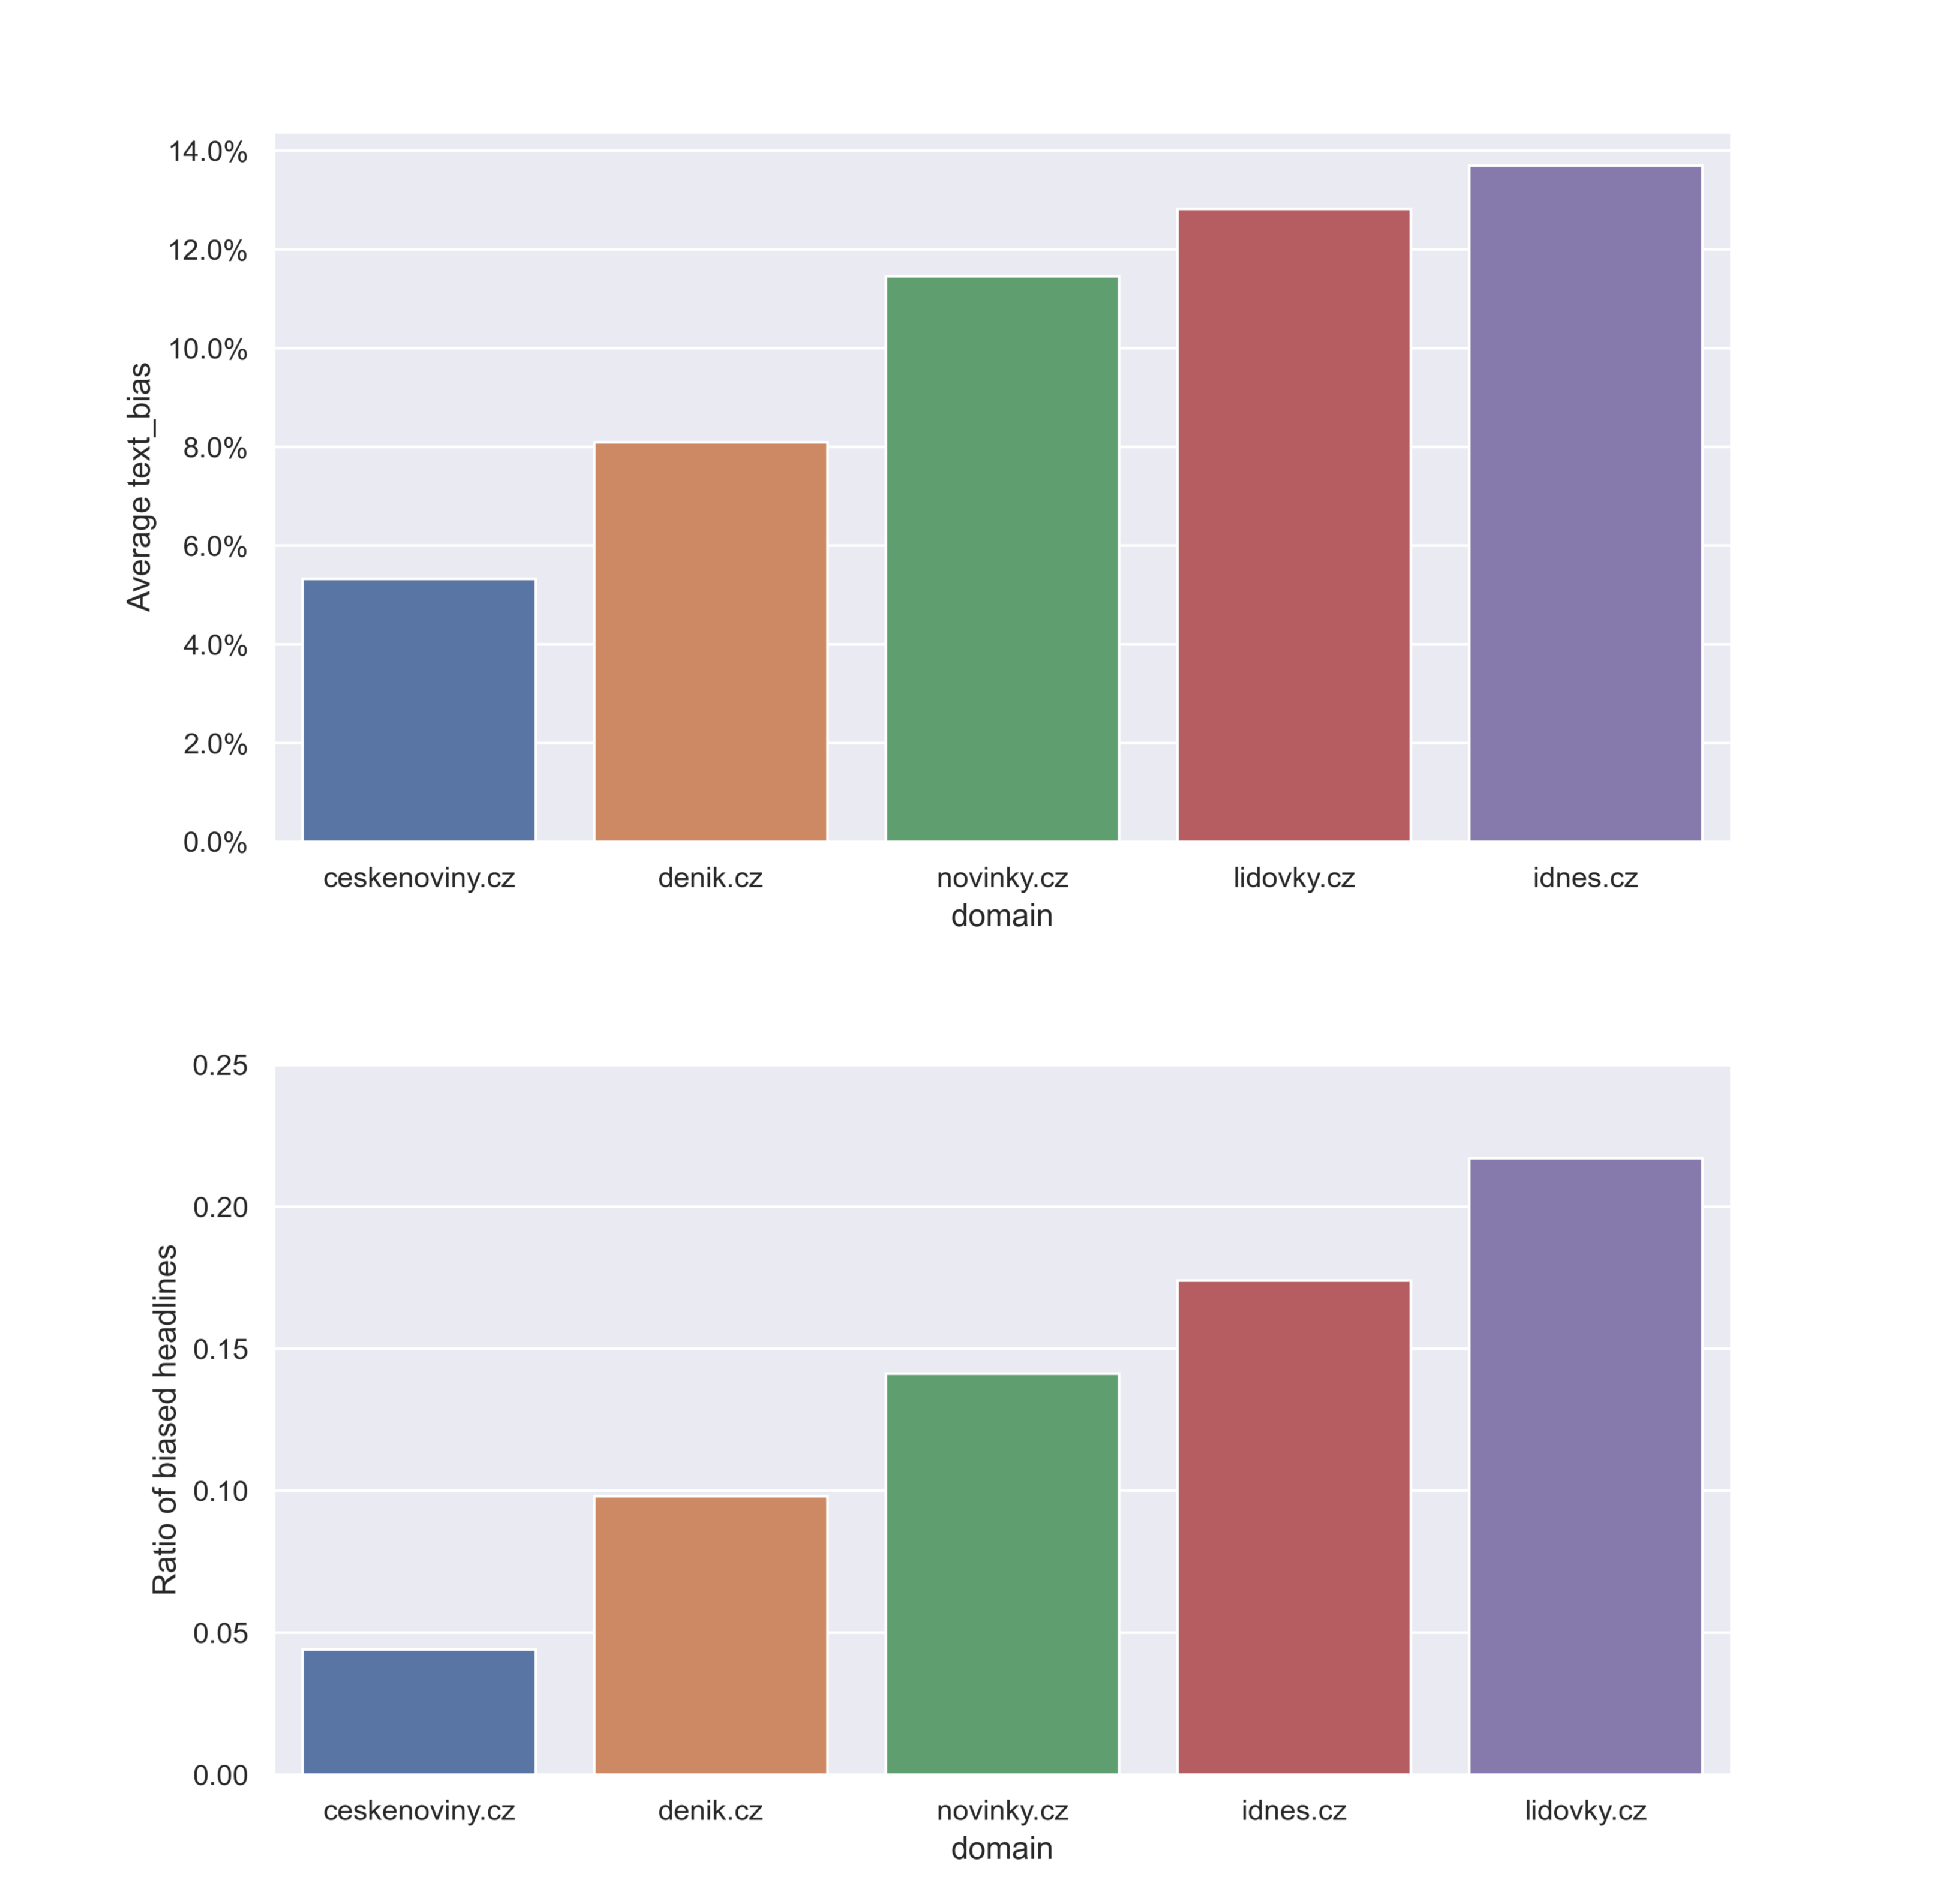
\includegraphics[scale=0.5]{my_modules/multimedia/inference/domains.jpg}
  \caption{Comparison of average text bias and headline bias across the domains.}
  \label{fig:domains}
}
\end{figure}



\tocless\subsection{Bias distribution}
As we can see in the prevous result, the average bias were in the interval between 5 and 15 percent. In the plots below, a precise distribution of bias in articles can be seen.
\ref{fig:dists}
\ref{fig:dists_ctk_idnes}

\begin{figure}[h]
\makebox[\textwidth][c]{
  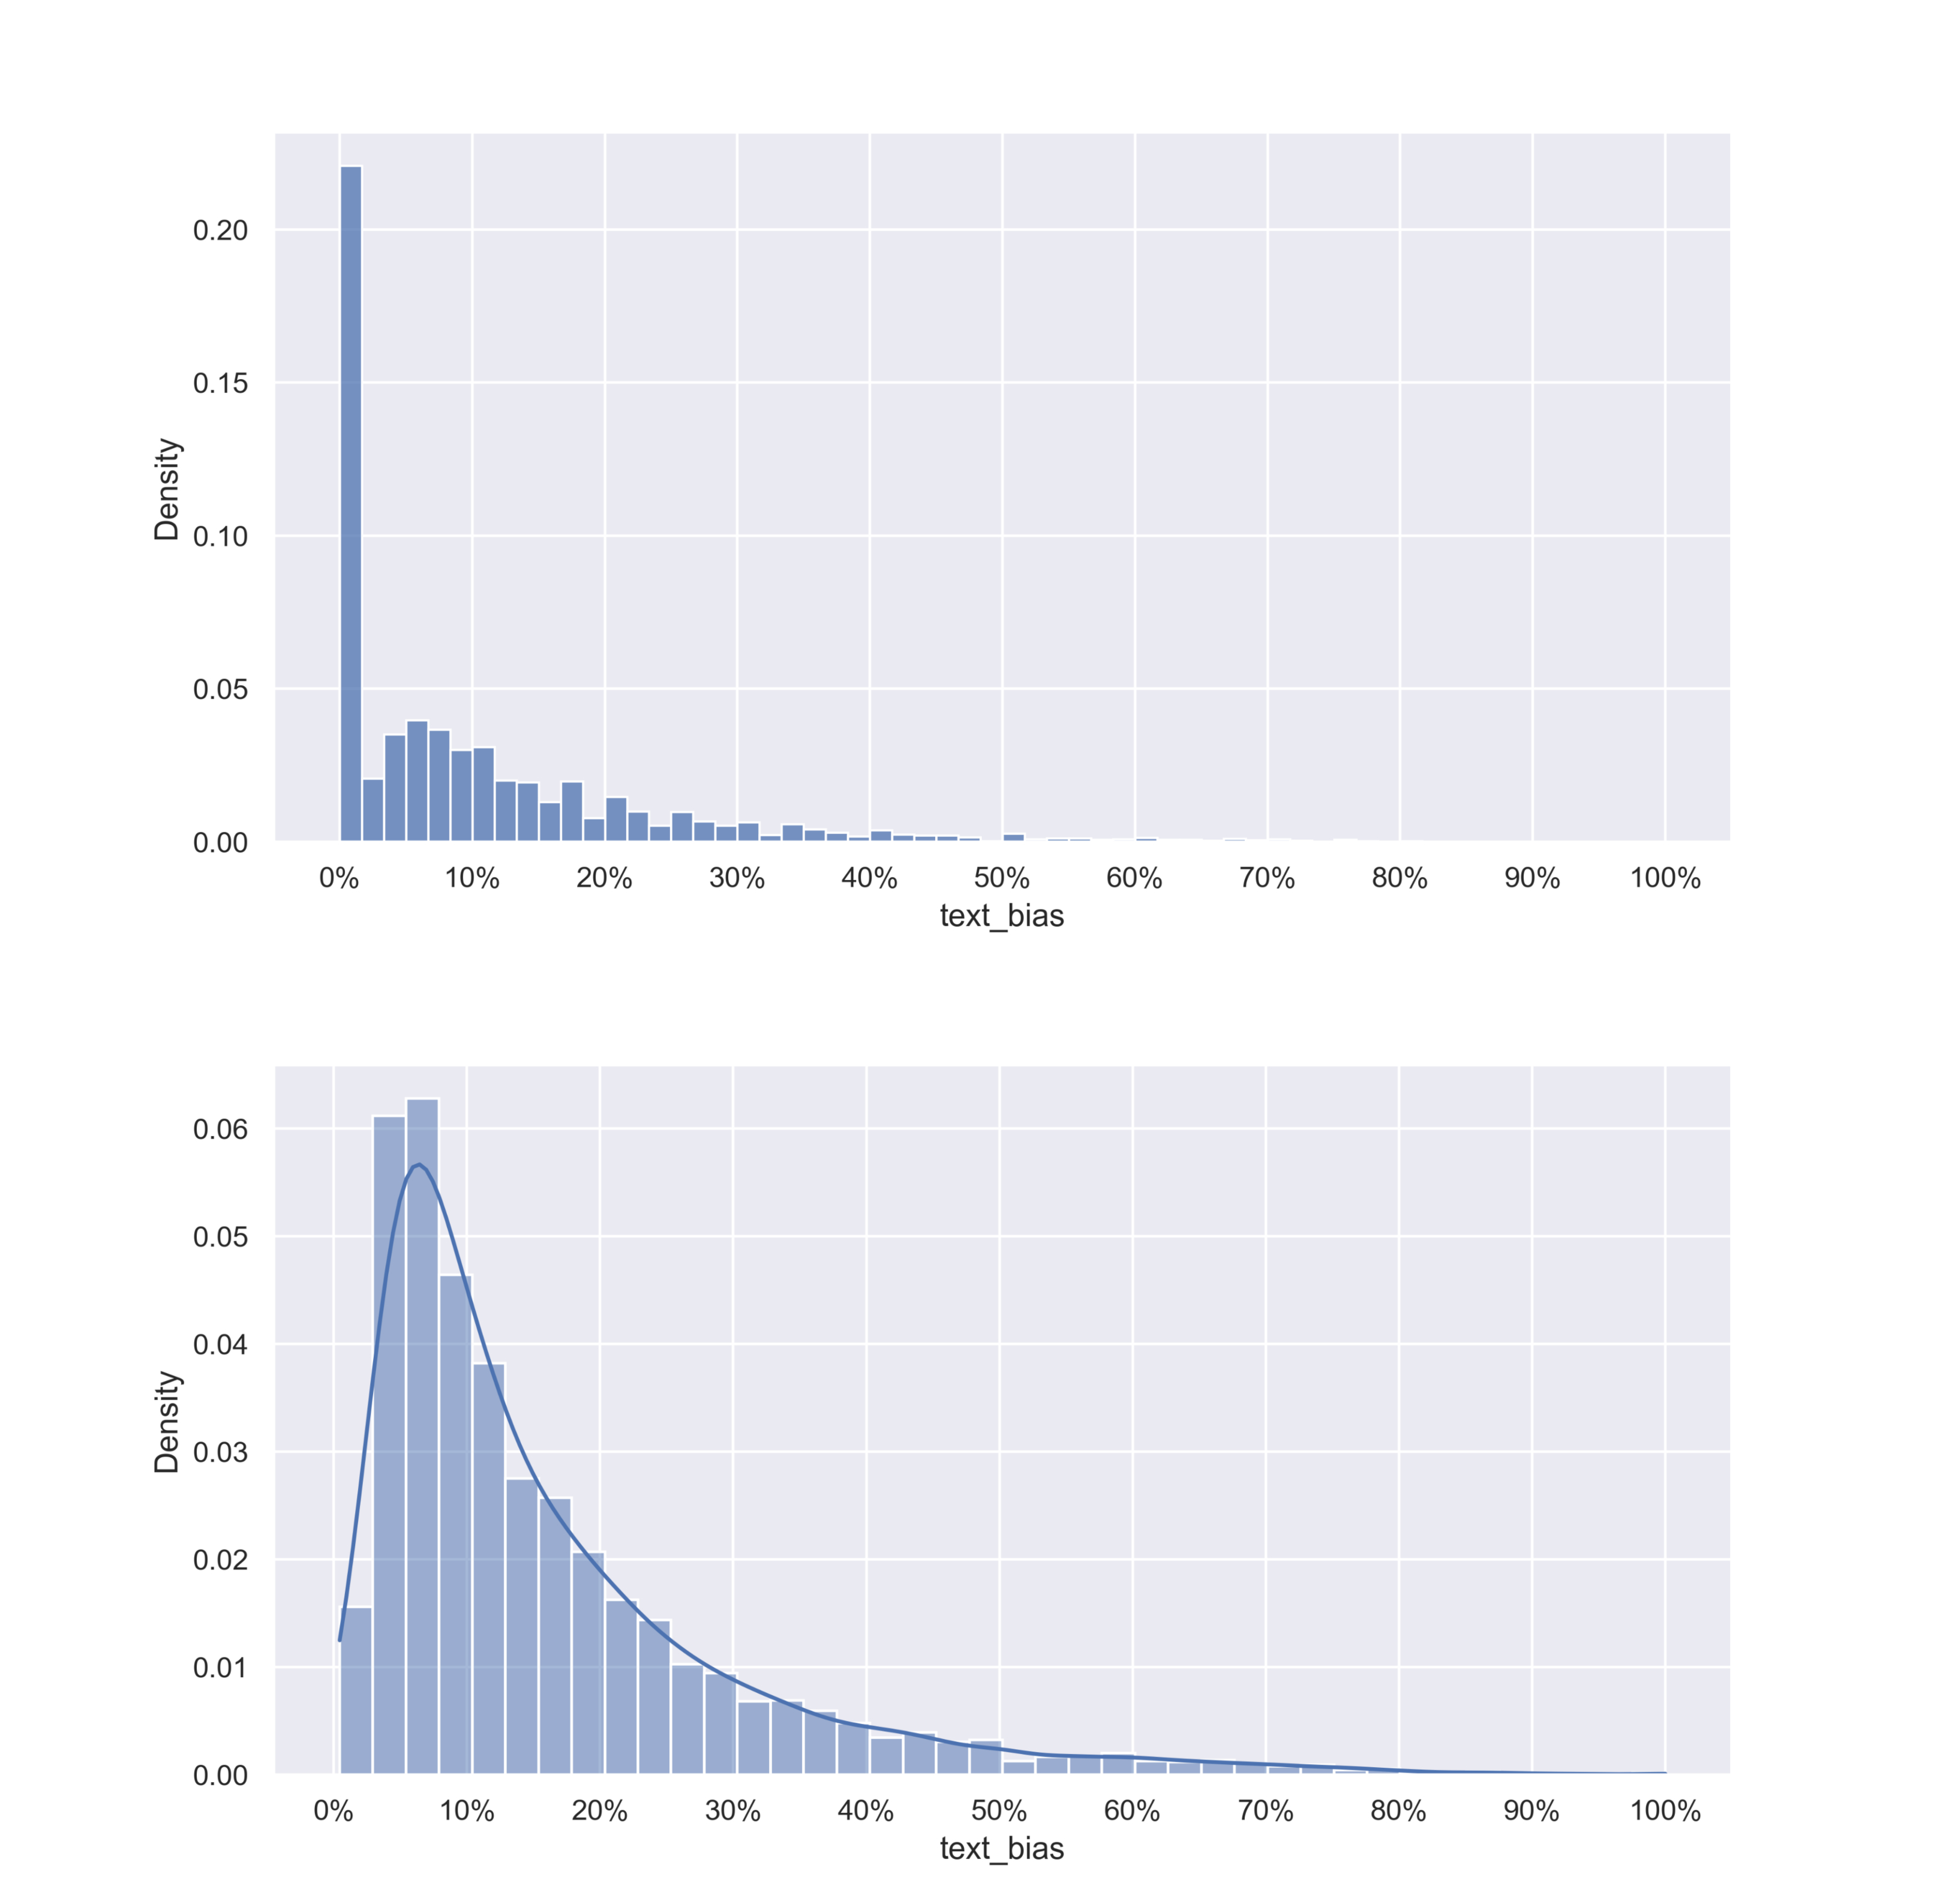
\includegraphics[scale=0.5]{my_modules/multimedia/inference/dists.jpg}
  \caption{Distribution of text bias values over the dataset. Second plot is without the articles with 0 text bias.}
  \label{fig:dists}
}
\end{figure}

\begin{figure}[h]
\makebox[\textwidth][c]{
  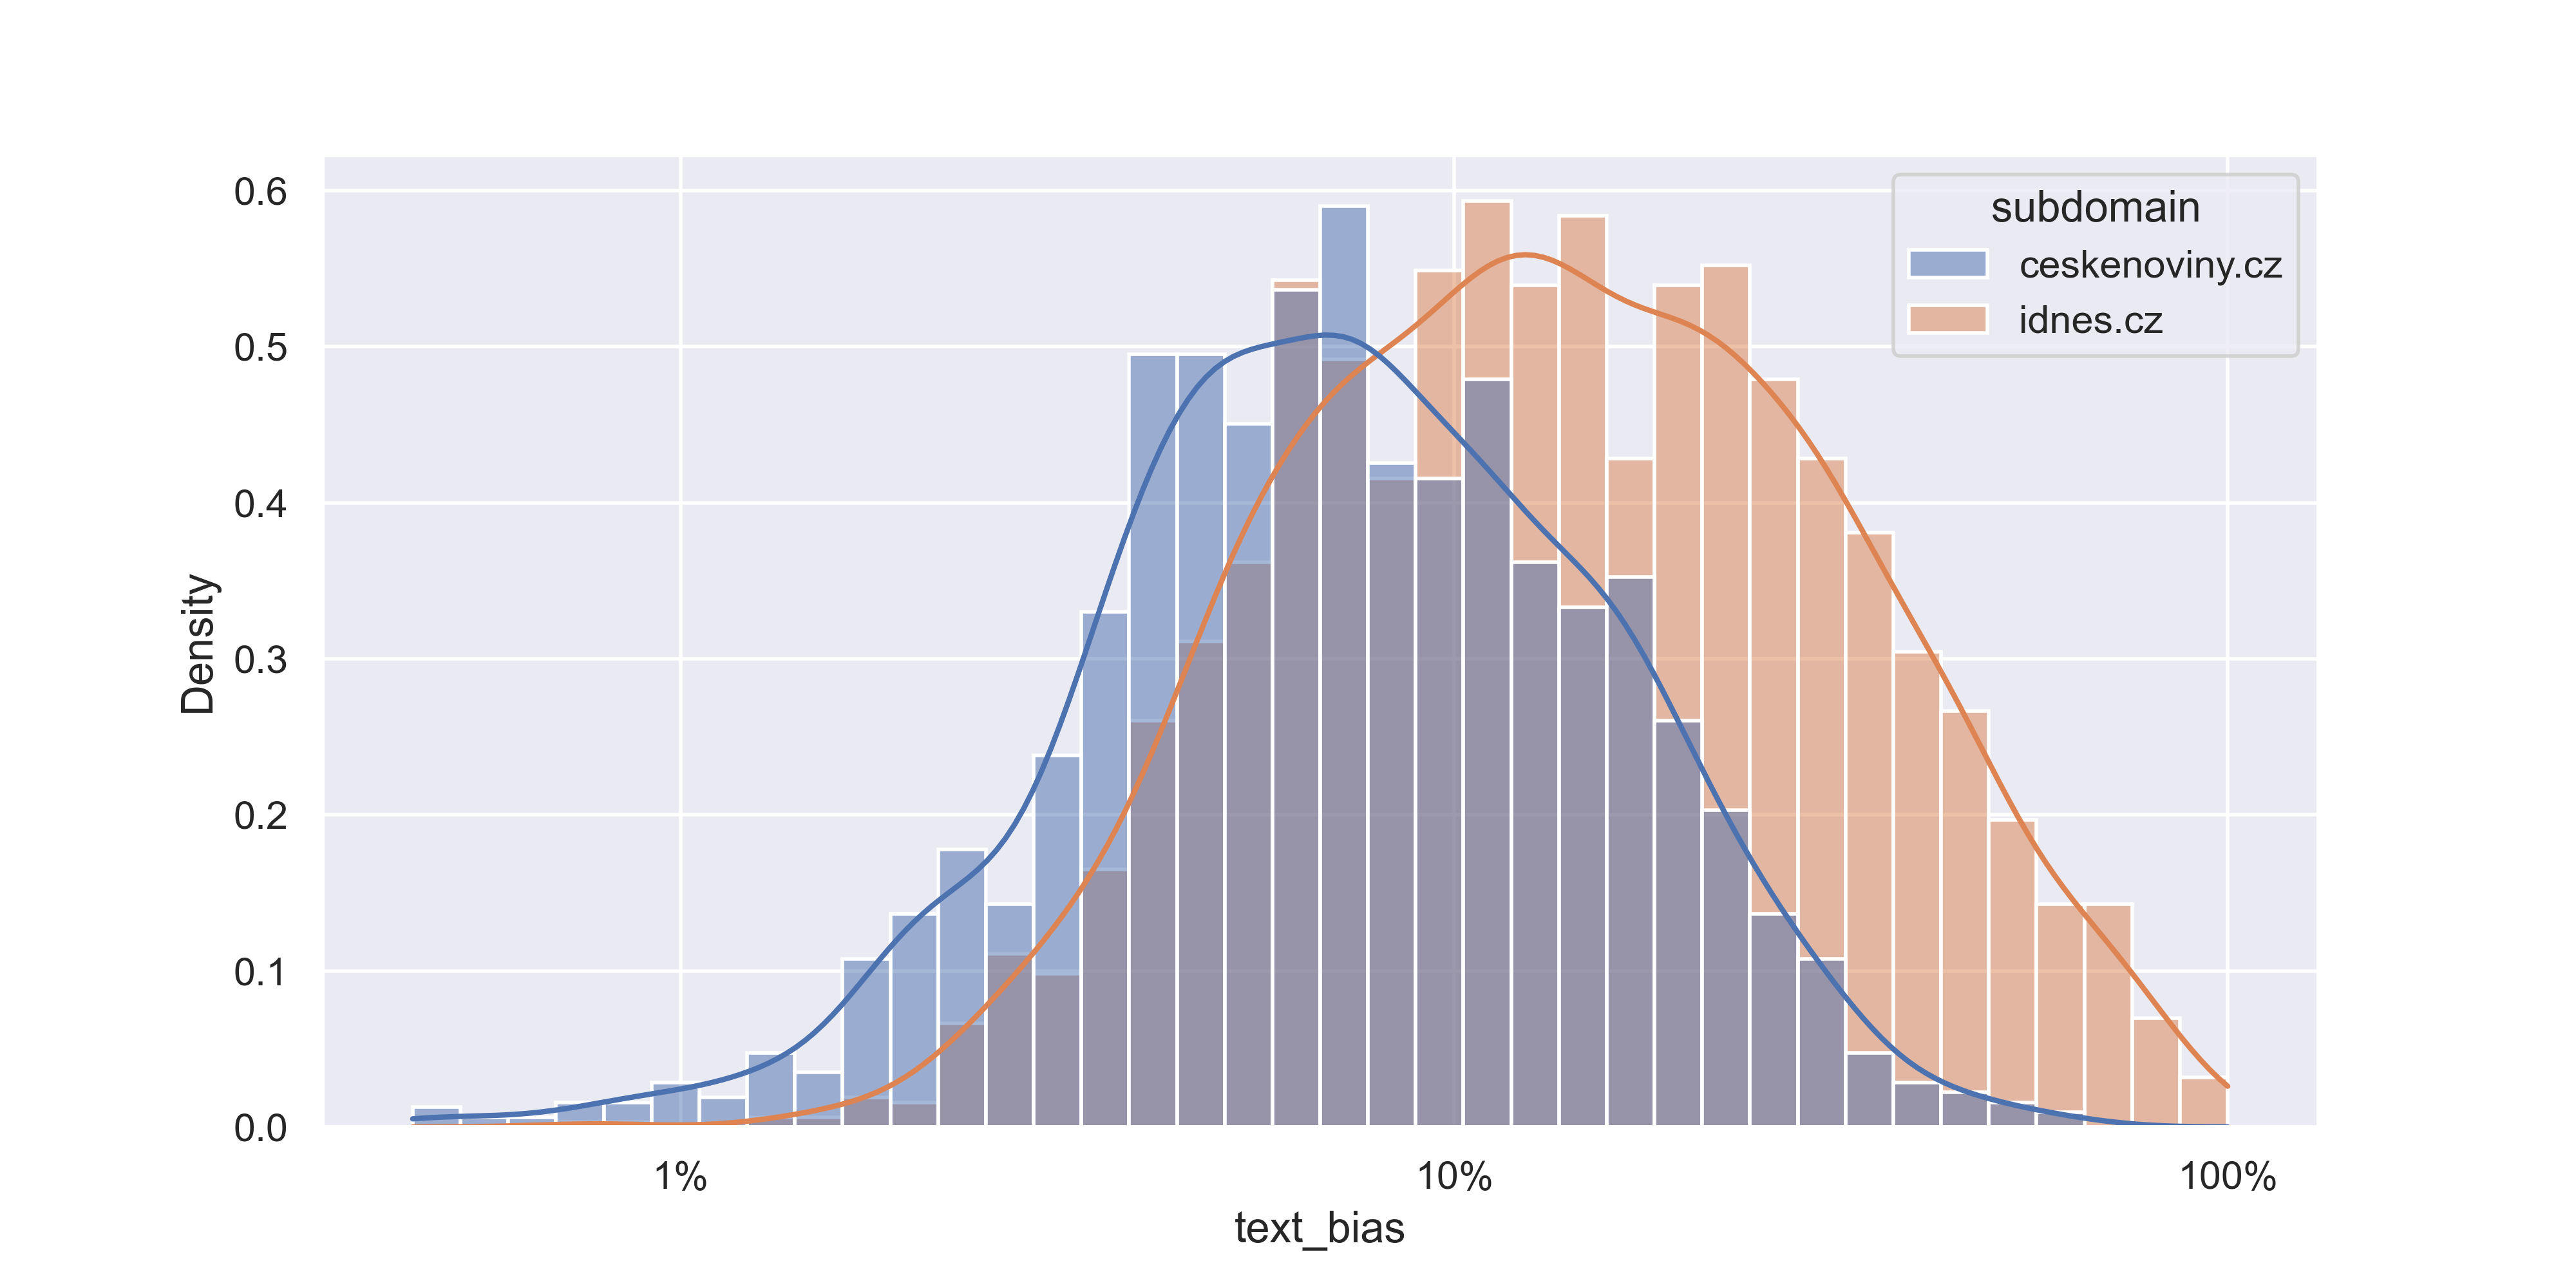
\includegraphics[scale=0.5]{my_modules/multimedia/inference/dists_ctk_idnes.png}
  \caption{Distributions of bias between two domains.}
  \label{fig:dists_ctk_idnes}
}
\end{figure}



\tocless\subsection{Correlations}
Correlation heatmap can be seen in
\begin{figure}[h]
\makebox[\textwidth][c]{
  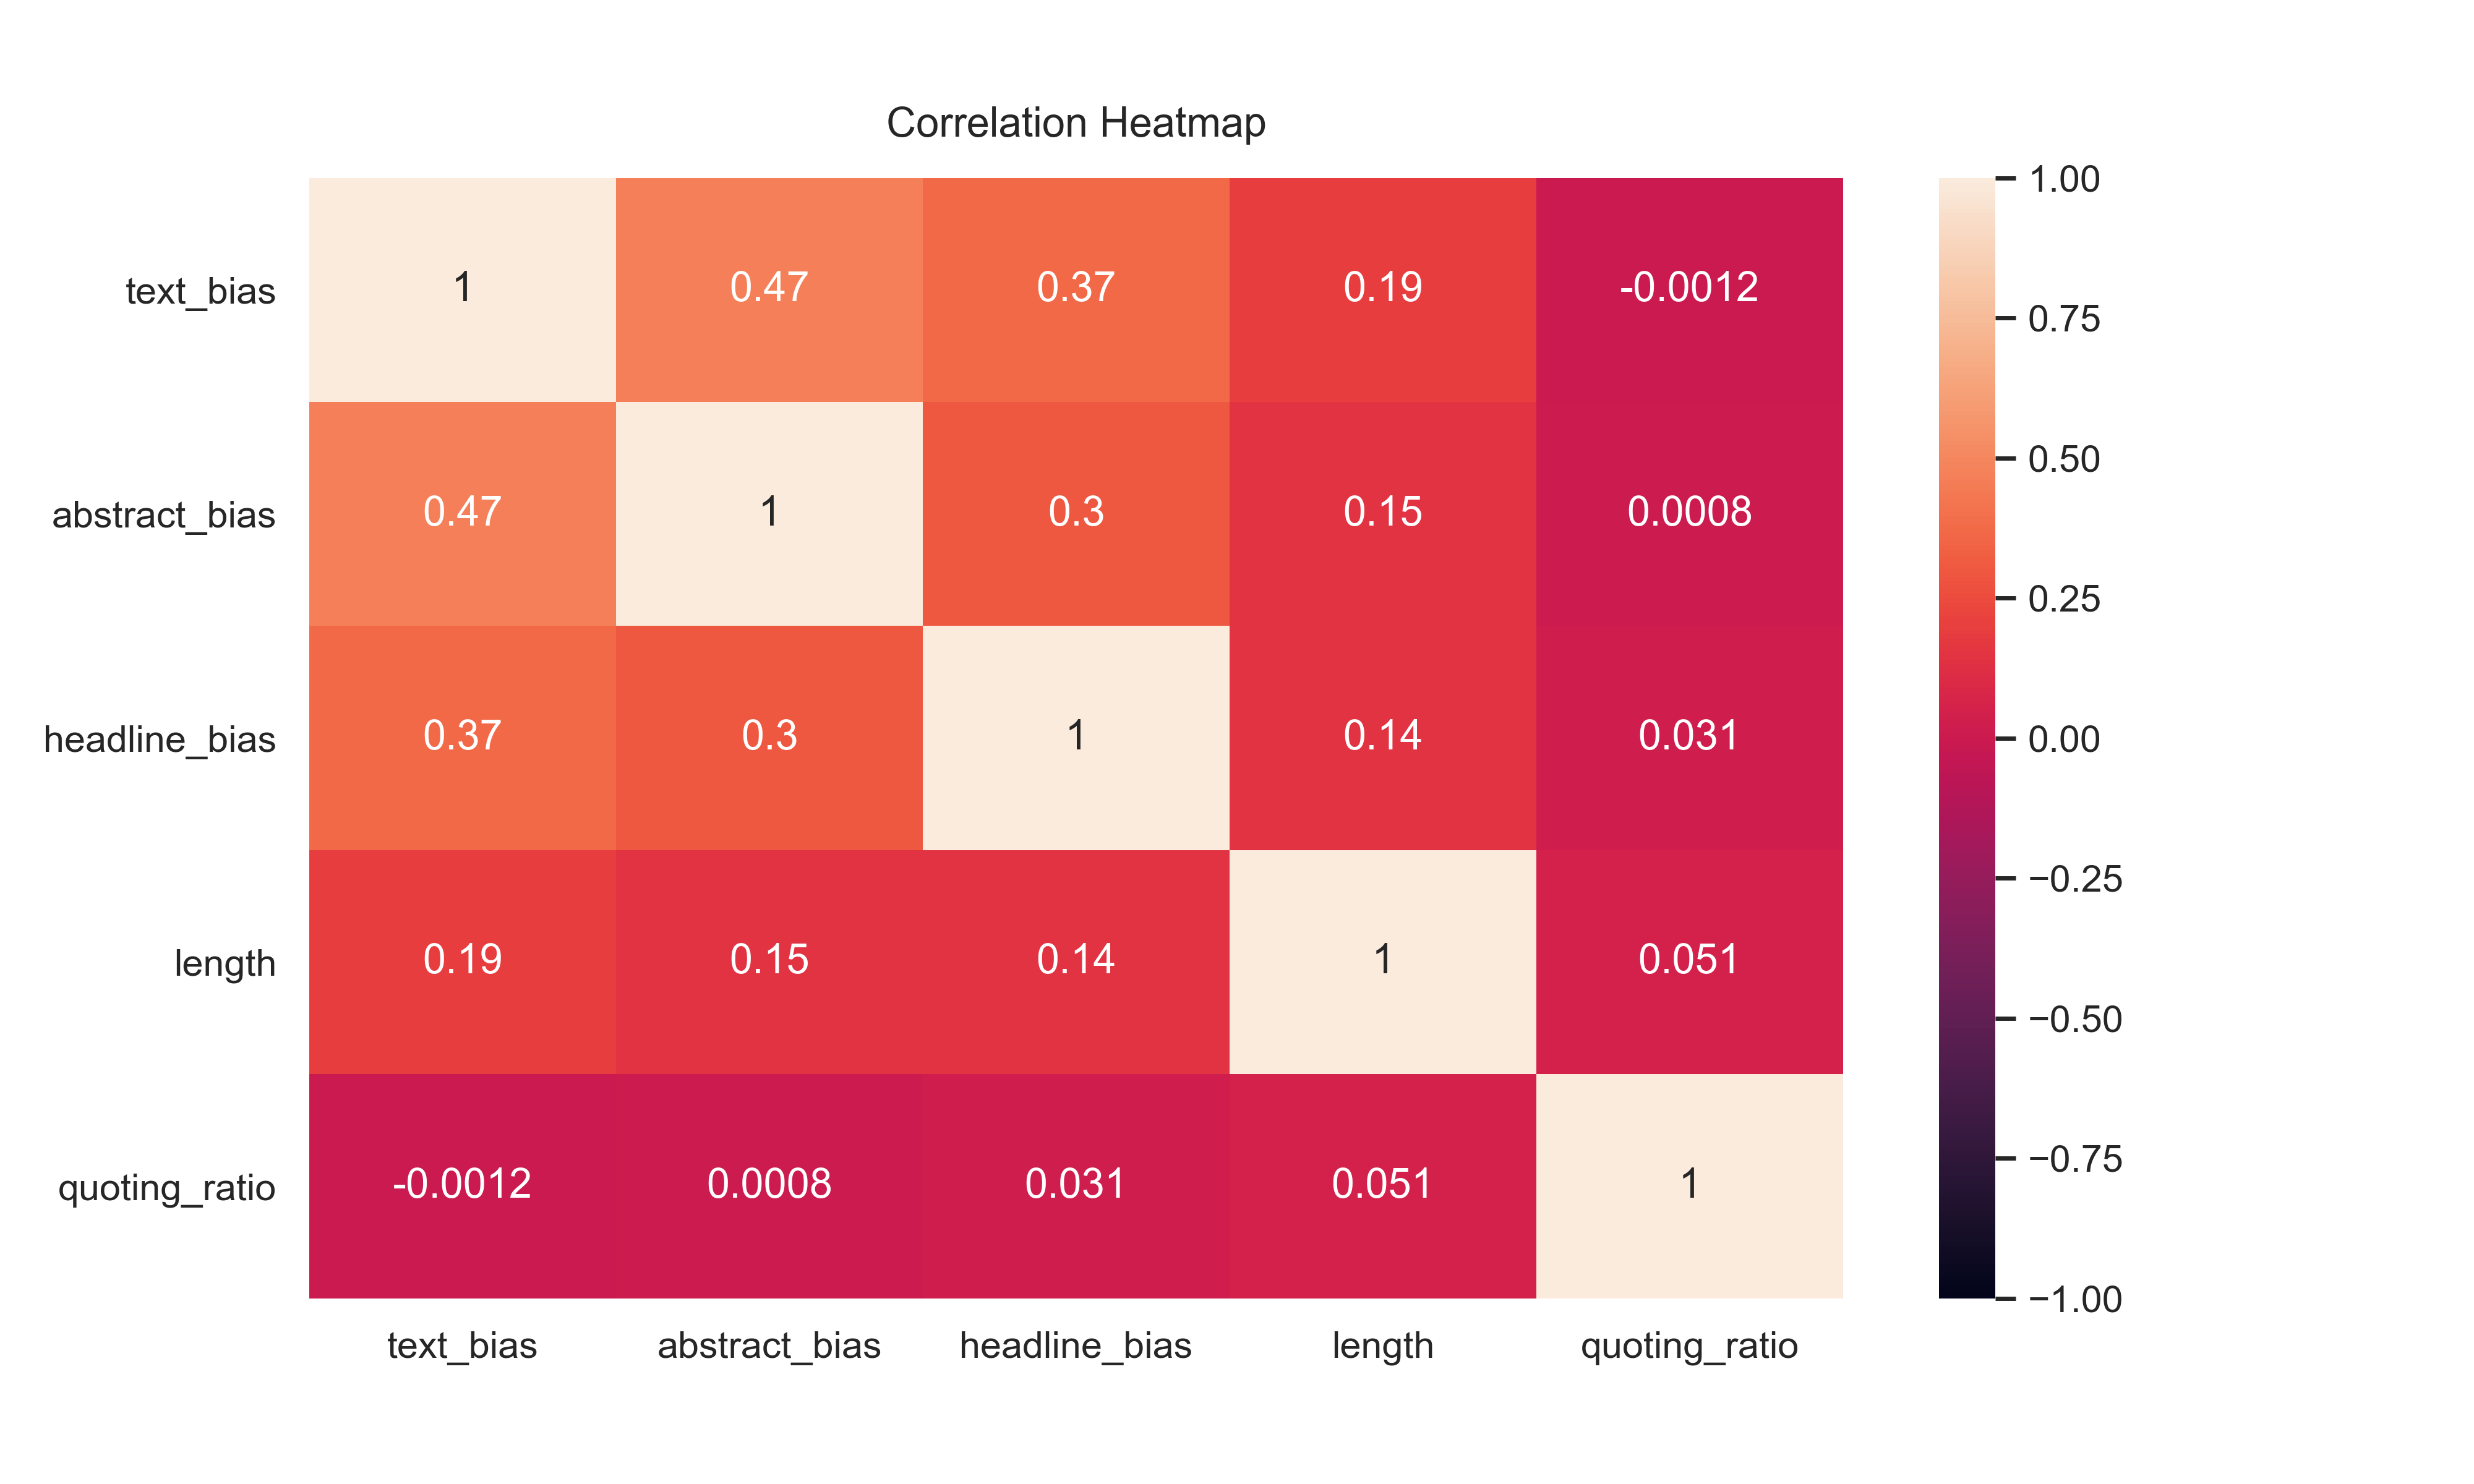
\includegraphics[scale=0.5]{my_modules/multimedia/inference/corr.png}
  \caption{Ten least and ten most biased sections.}
  \label{fig:corr}
}
\end{figure}


\tocless\subsection{Bias along sections}
commentary wins

\begin{figure}[h]
\makebox[\textwidth][c]{
  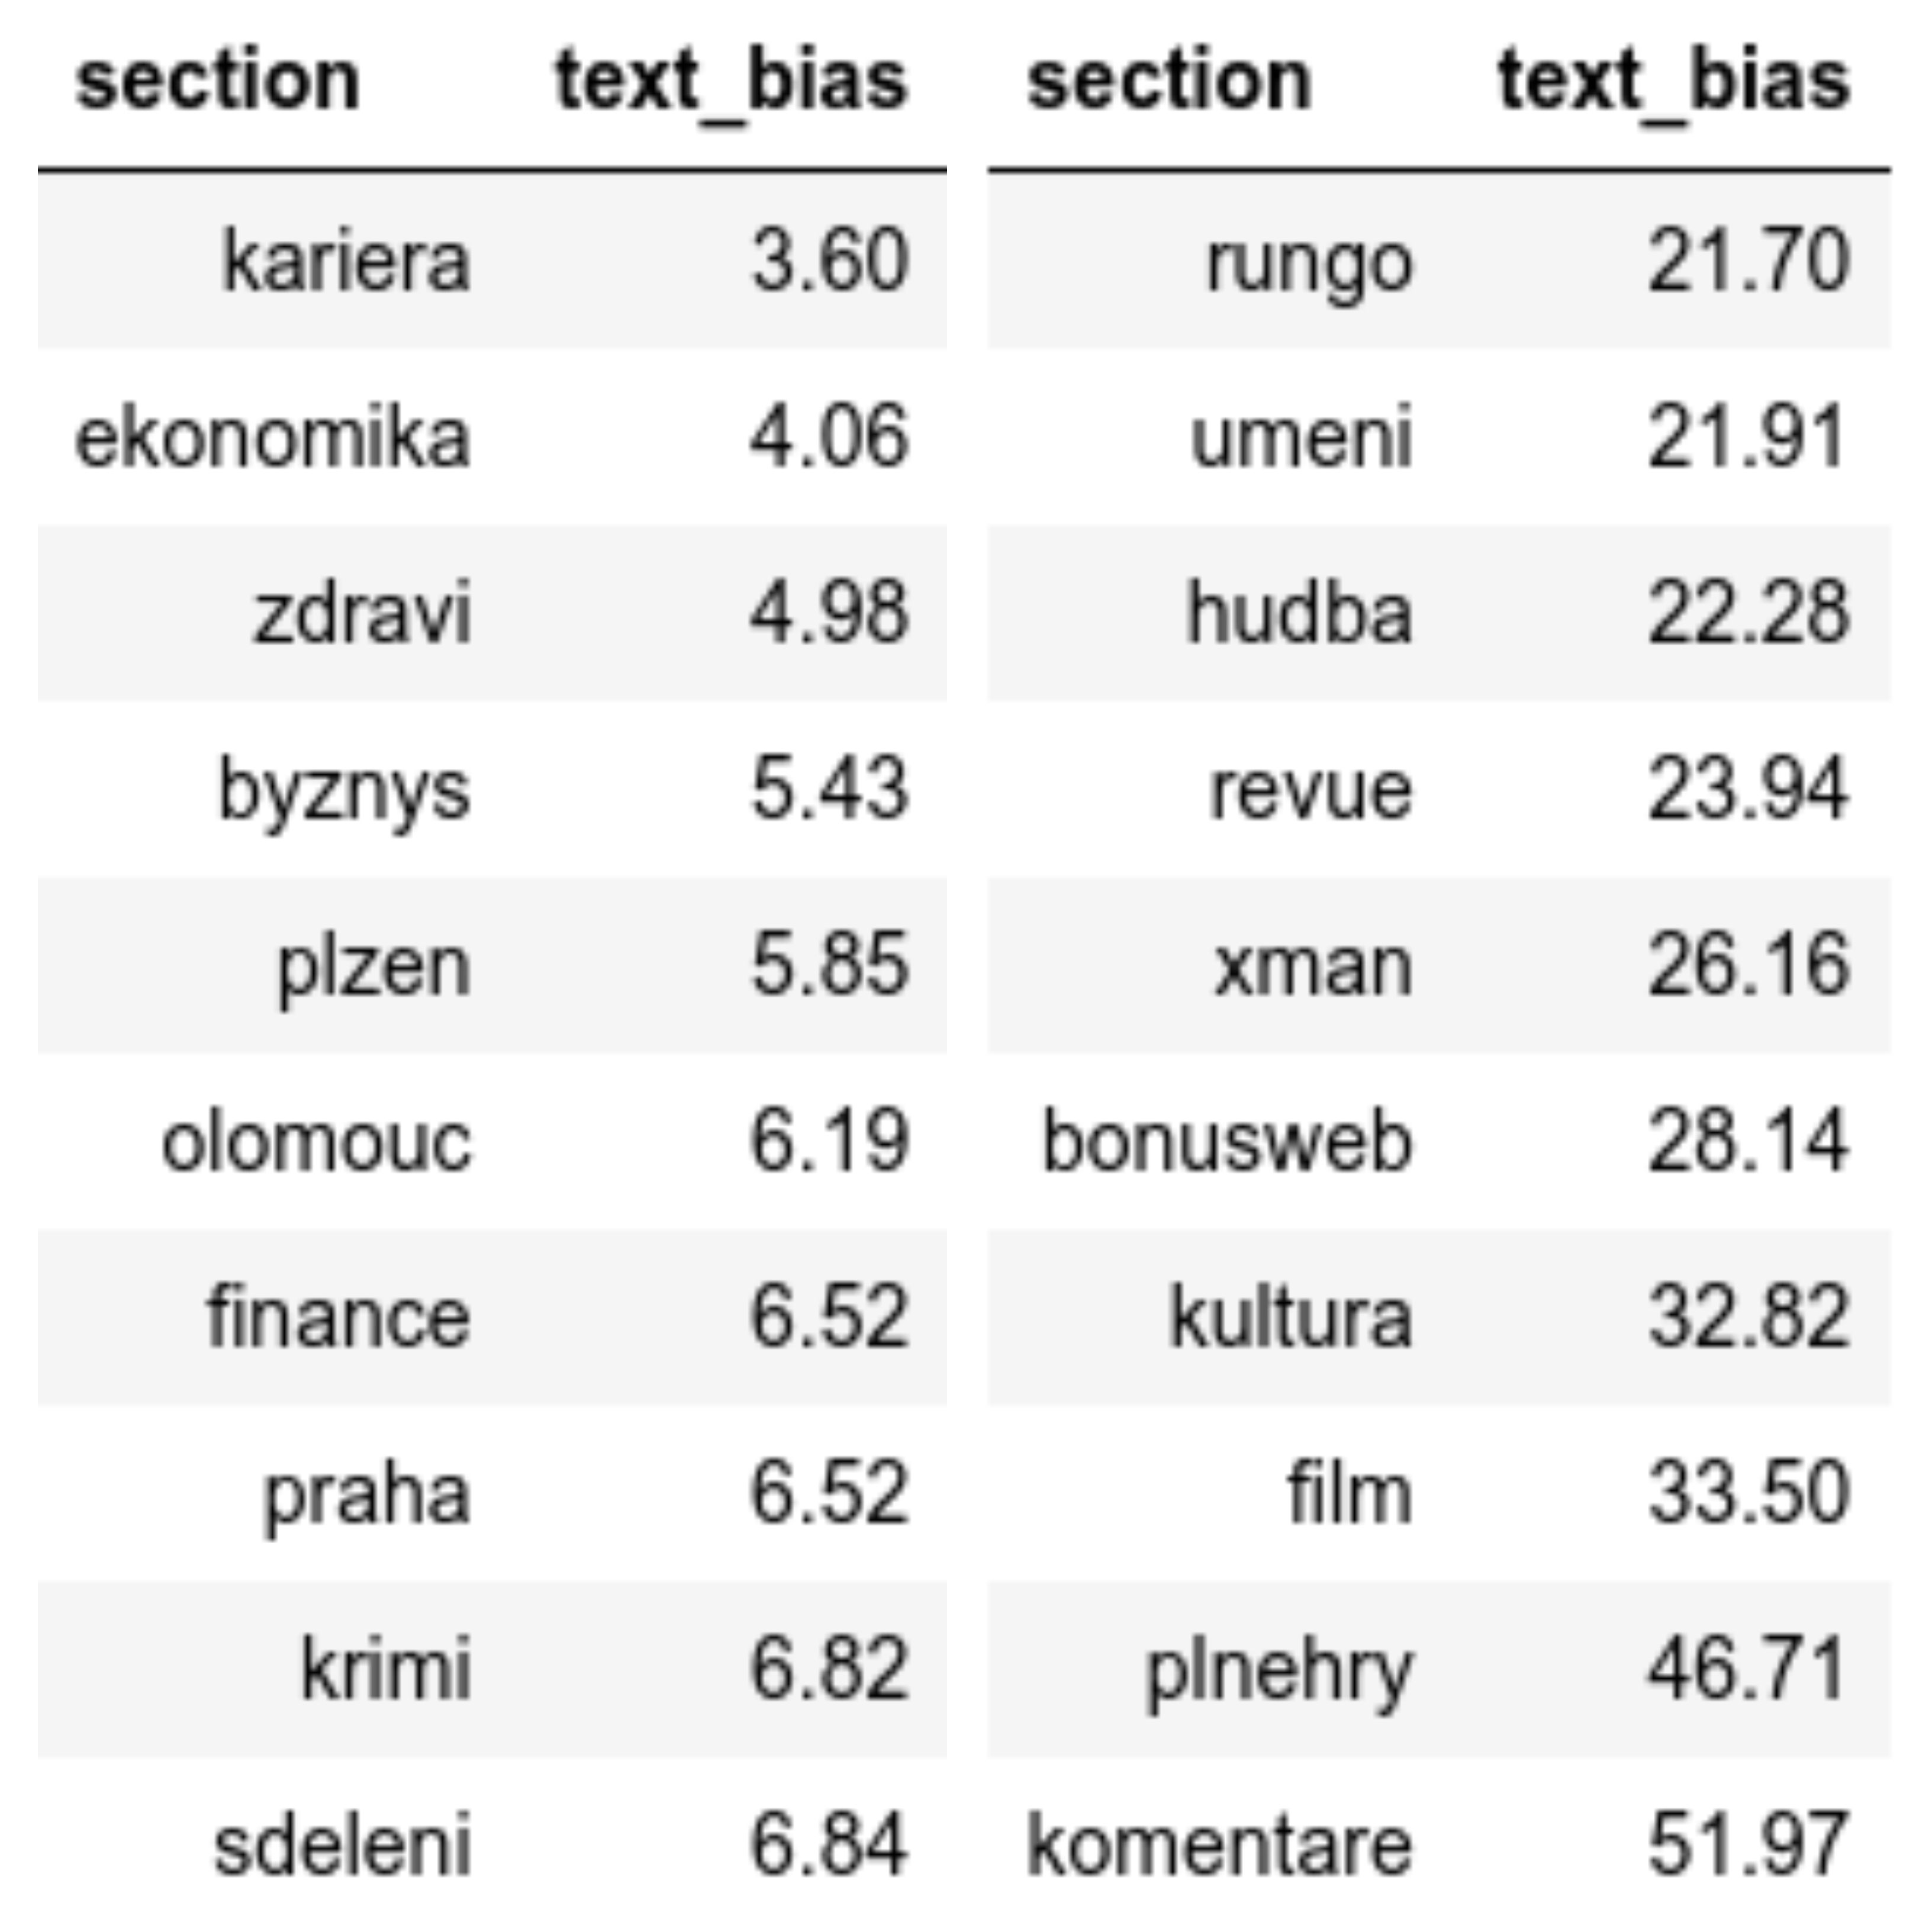
\includegraphics[scale=0.2]{my_modules/multimedia/inference/sections.jpg}
  \caption{Ten least and ten most biased sections.}
  \label{fig:sections}
}
\end{figure}


%%%%%%%%%%%%%%%%%%%%%%%%%%%%%%%% DENIK %%%%%%%%%%%%%%%%%%%%%%%%%%%%%%%%%%%%%%%%%%%%%%

\tocless\subsection{Denik.cz experiments}
on CTK there were only data in years 2016 and 2017. so no time plot

\begin{figure}[h]
\makebox[\textwidth][c]{
  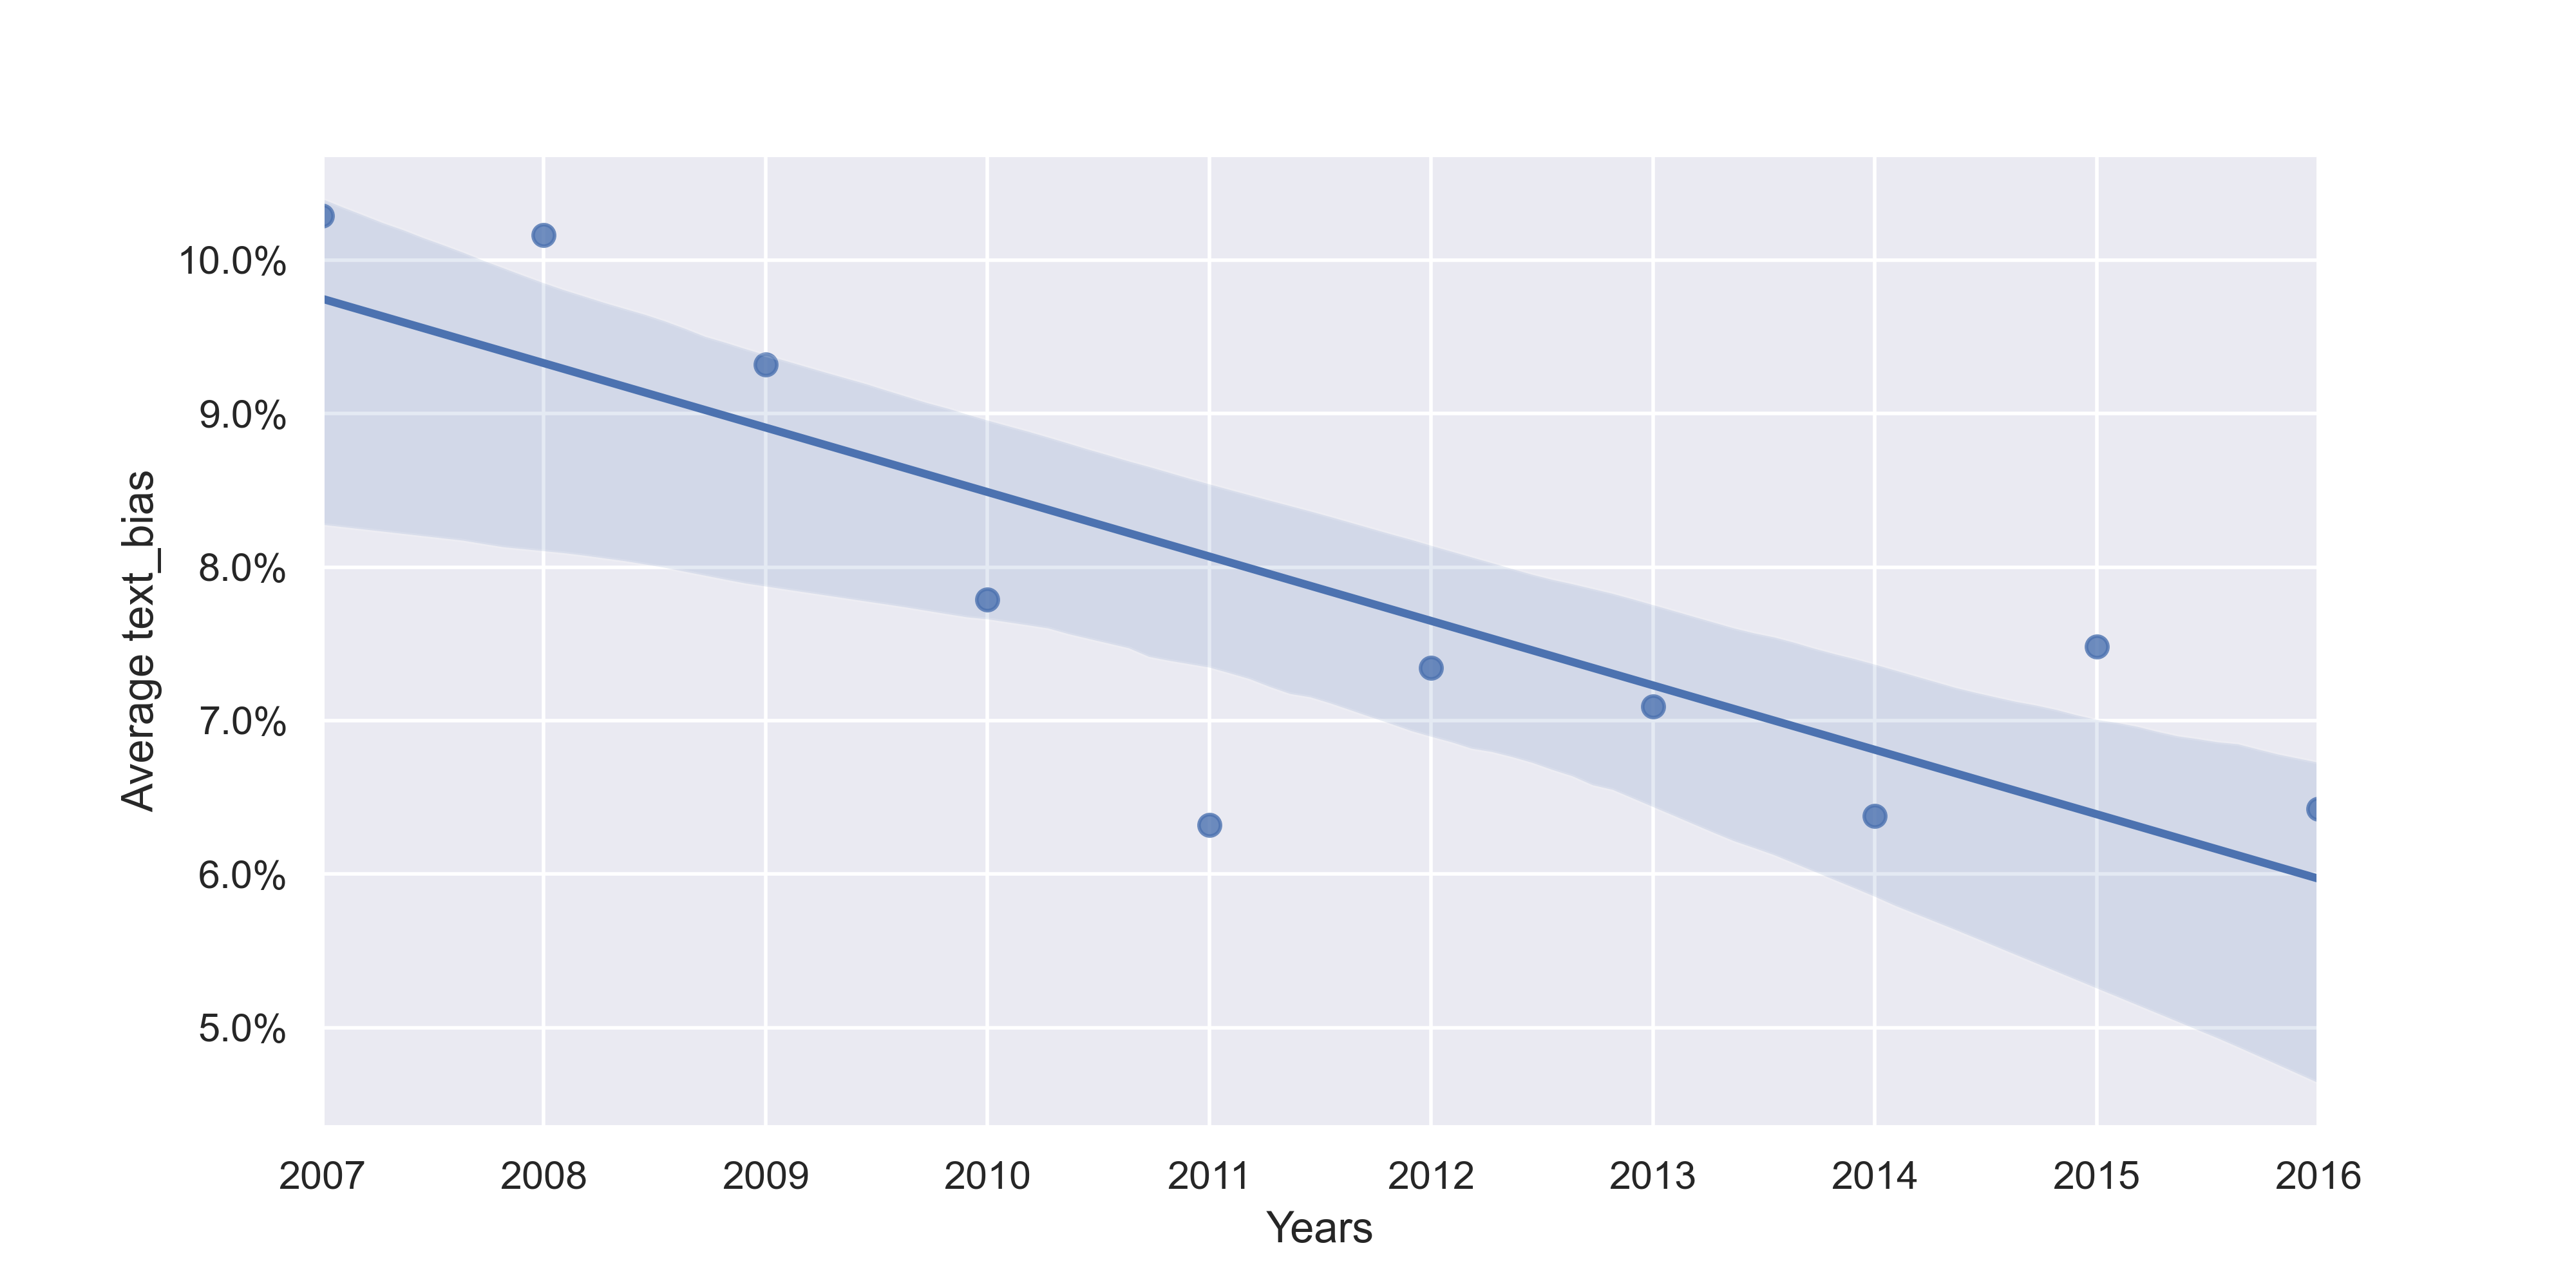
\includegraphics[scale=0.5]{my_modules/multimedia/inference/denik_years.png}
  \caption{Distributions of bias between two domains.}
  \label{fig:denik_years}
}
\end{figure}


\begin{figure}[h]
\makebox[\textwidth][c]{
  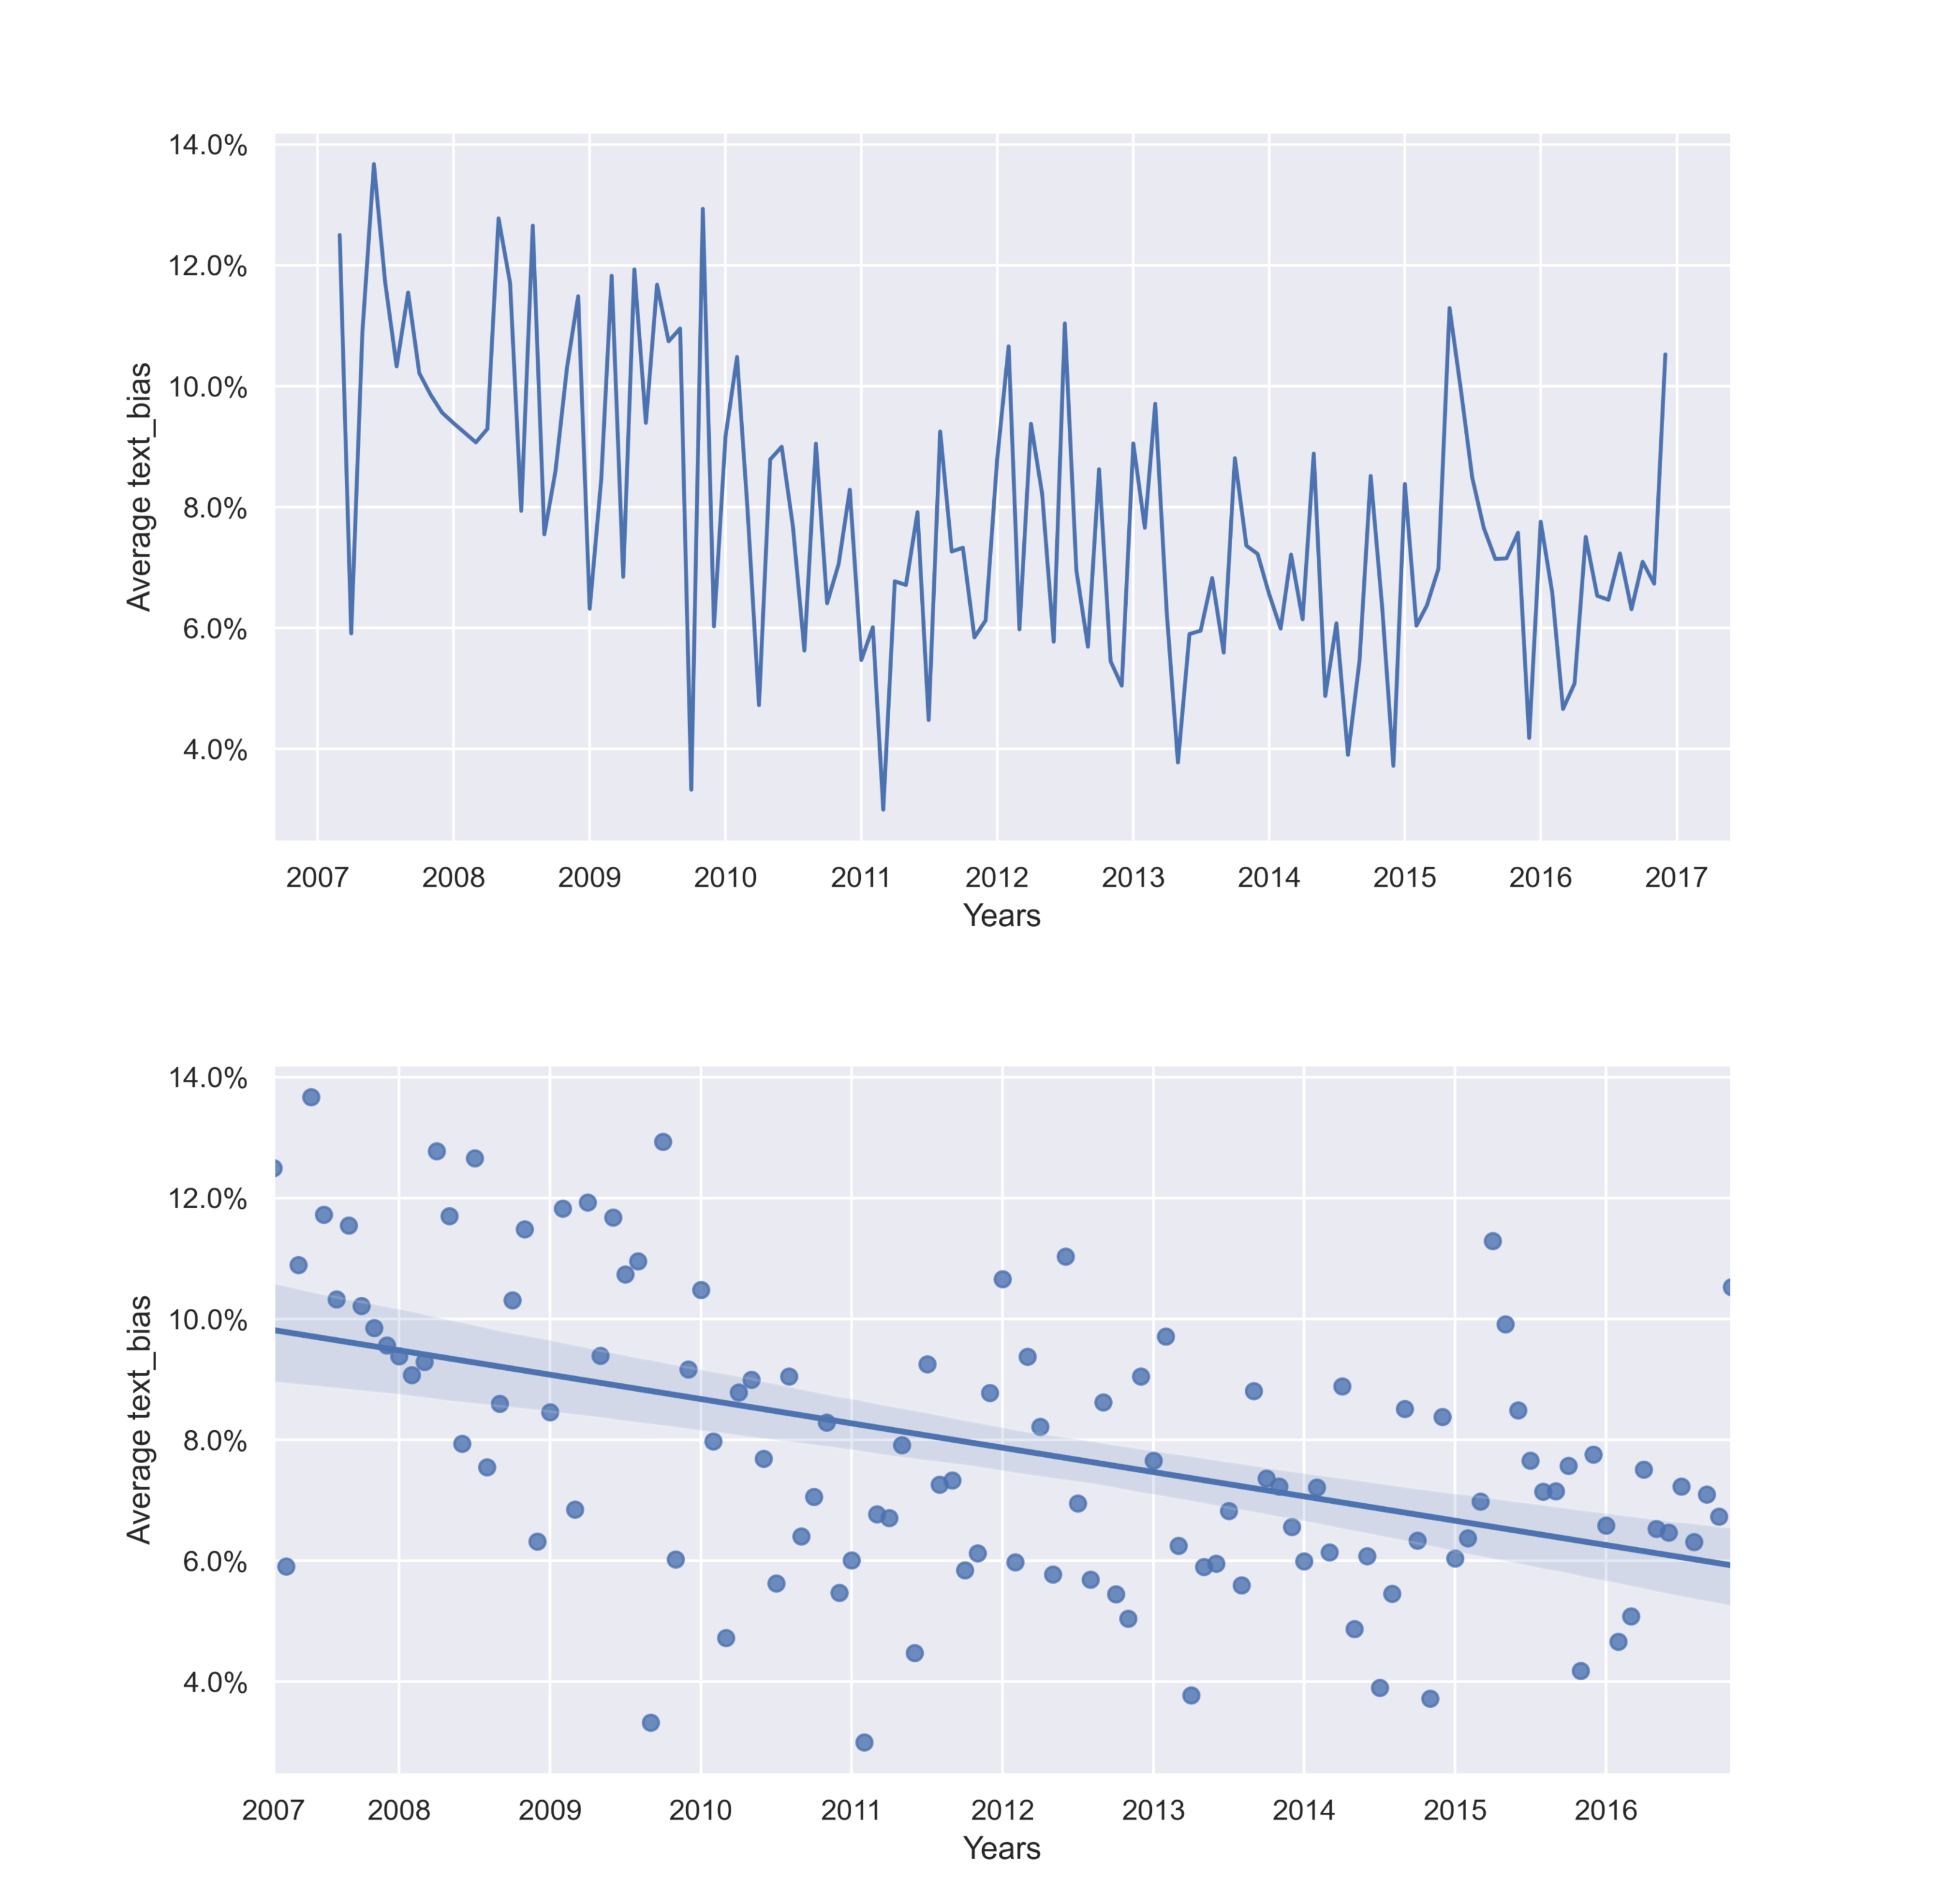
\includegraphics[scale=0.5]{my_modules/multimedia/inference/months_clean.jpg}
  \caption{Distributions of bias between two domains.}
  \label{fig:months_clean}
}
\end{figure}







%%%%%%%%%%%%%%%%%%%%%%%%%%%%%%%% APP %%%%%%%%%%%%%%%%%%%%%%%%%%%%%%%%%%%%%%%%%%%%%%%%%%%%%%%%%%%%%%%

\section{Application}
Additionally, I provide a simple web demo application for the reader to experiment with\footnote{\url{https://huggingface.co/spaces/horychtom/czech_media_bias_detection}}. The app runs on HuggingFace's spaces\footnote{\url{https://huggingface.co/spaces}} which is a free hosting service for demonstraing \gls{ml} applications. For the frontend, Gradio\footnote{\url{https://gradio.app/}} was used.

The user can insert arbitrary text in Czech language (text in other languages will result in meaningless outcomes). The text is then split into sentences and classified individually.

The app shows results in two output windows; first one \textit{classification} displays inserted text with highlighted labels. Second one, \textit{ratio}, displays ratio of biased/unbiased sentences in the text.

Example can be seen in figure \ref{fig:demodemo}.

\begin{figure}[H]
\makebox[\textwidth][c]{
  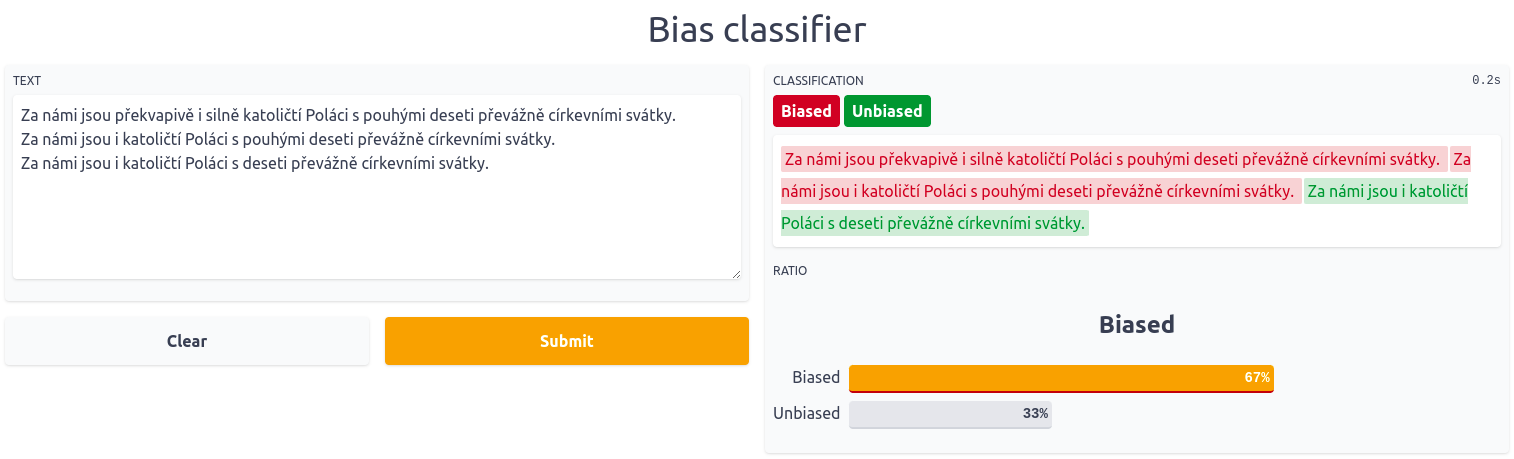
\includegraphics[scale=0.3]{my_modules/multimedia/bias.png}
  \caption{Example of the bias classifier demo usage.}
  \label{fig:demodemo}
  }
\end{figure}




\section{Discussion}
Not all commentary articles are marked in the data.
Sometimes quoting is not marked, no discussion etc.
An example of classified news article can be seen in Appendix \ref{classified_article}.

